\documentclass[./main.tex]{subfiles}

\begin{document}
\renewcommand{\thesubsubsection}{{\color{red}C\arabic{subsubsection}}}

\subsection{Obtención del software de Oracle y configuración de Red}\label{sec:obtenc-del-soft}
Descargamos la base de datos de
\href{https://www.oracle.com/database/technologies/oracle-database-software-downloads.html}
{la página de descargas de Oracle} (el cual requiere registro previo), lo descargamos y lo
transferimos a la máquina virtual.
\begin{codeC}{shell-session}{Sesión de shell transfiriendo archivo}
$ scp -P 2222 Descargas/LINUX.X64_193000_db_home.zip candrade@127.0.0.1:/home/candrade/Descargas/
candrade@127.0.0.1's password:
LINUX.X64_193000_db_home.zip                                                          100% 2918MB  44.2MB/s   01:05
\end{codeC}

% $

Mientras se transfiere/descarga el software, podemos manipular la red, anteriormente se usaba una
red NAT entre la máquina anfitriona y la huésped. Ahora vamos a conectarla con un adaptador puente
en VirtualBox, en la configuración de la red en la pestaña \textit{Adaptador 1} seleccionamos
Adaptador puente y elegimos la red que esta conectada a internet, en este caso \texttt{enp3s0}\footnote{Puede
  cambiar dependiendo del estado de la máquina anfintrion}
\begin{figure}[H]
  \centering
  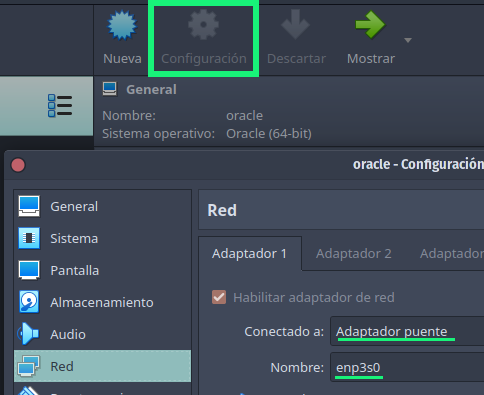
\includegraphics[width=\columnwidth]{red}
  \caption{Configuración de red de la VM}\label{fig:red}
\end{figure}

Conectamos la VM a la red si se desconecto, con \texttt{ip a} en la VM
\begin{codeC}{shell-session}{Fragmento del comando \texttt{ip a} en la VM}
2: enp0s3: <BROADCAST,MULTICAST,UP,LOWER_UP> mtu 1500 qdisc fq_codel state UP group default qlen 1000
    link/ether 08:00:27:fa:6f:2e brd ff:ff:ff:ff:ff:ff
    inet 192.168.0.103/24 brd 192.168.0.255 scope global dynamic noprefixroute enp0s3
\end{codeC}

Vemos que la ip que se le asignó a nuestra VM es $192.168.0.103$, sabiendo que la máquina anfintriona
tiene la ip $192.168.0.107$, procedemos a añadir dichas máquinas en los archivos \texttt{/etc/hosts}
con sus respectivos \texttt{hostsnames}
\begin{codeCL}{bash}{Texto que se insertó en \texttt{/etc/hosts} en la MA}{src:hosts-vm}
192.168.0.103 oraclebdd oraclebdd.fi.unam
\end{codeCL}
\begin{codeCL}{bash}{Texto que se insertó en \texttt{/etc/hosts} en la VM}{src:hosts-vm}
127.0.1.1 oraclebdd oraclebdd.unam.mx oraclebdd.fi.unam

192.168.0.107 Arch-R7
\end{codeCL}

\subsubsection{Salida del Comando Ping}\label{sec:salida-del-comando}
\begin{figure}[H]
  \centering
  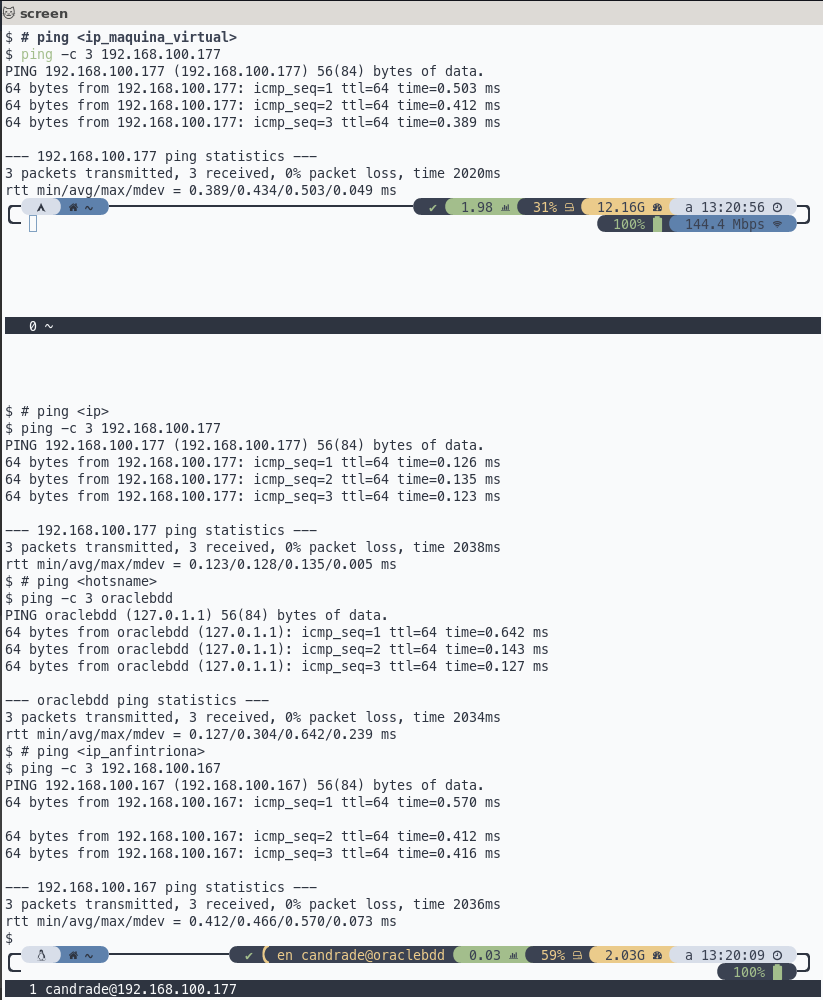
\includegraphics[width=\columnwidth]{ping}
  \caption{C1. Salida del Comando Ping}\label{fig:ping}
\end{figure}

Una vez descargado el archivo mencionado al principio de la subsección lo extraemos:
\begin{codeC}{shell-session}{Commando para extraer un archivo \texttt{zip}}
$ unzip -q LINUX.X64_193000_db_home.zip -d ./LINUX.X64_193000_db_home
\end{codeC}
Actualizamos e instalamos las bibliotecas necesarias como usuario administrador%$
\begin{codeC}{shell-session}{Comando para instalar bibliotecas faltantes}
# dnf install -y bc binutils elfutils-libelf elfutils-libelf-devel fontconfig-devel glibc glibc-devel ksh libaio libaio-devel libXrender libX11 libXau libXi libXtst libgcc libnsl librdmacm libstdc++ libstdc++-devel libxcb libibverbs make policycoreutils policycoreutils-python-utils smartmontools sysstat unixODBC
\end{codeC}

Configuramos los parametros del kernel.
\begin{codeC}{bash}{\texttt{97-oracle-database-sysctl.conf}}
# lineas agregadas para Oracle

fs.aio-max-nr = 1048576
fs.file-max = 6815744
kernel.shmall = 2097152
kernel.shmmax = 4294967295
kernel.shmmni = 4096
kernel.sem = 250 32000 100 128
net.ipv4.ip_local_port_range = 9000 65500
net.core.rmem_default = 262144
net.core.rmem_max = 4194304
net.core.wmem_default = 262144
net.core.wmem_max = 1048576
\end{codeC}

y después ejecutar el siguiente comando \texttt{/sbin/sysctl -p}.

Ahora agregamos las siguientes líneas al final del archivo \texttt{/etc/security/limits.conf}
\begin{codeC}{bash}{\texttt{/etc/security/limits.conf}}
#lineas agregadas requeridas para oracle
oracle soft nofile 1024
oracle hard nofile 65536
oracle soft nproc 2047
oracle hard nproc 16384
oracle soft stack 10240
oracle hard stack 32768
oracle hard memlock 134217728
oracle soft memlock 134217728
\end{codeC}
\newpage{}
Creamos los siguientes grupos
\begin{codeC}{shell-session}{Grupos a añadir}
# groupadd -g 54321 oinstall
The memcache was not invalidated by NSS responder.
# groupadd -g 54322 dba
# groupadd -g 54323 oper
# groupadd -g 54321 oinstall
\end{codeC}

Creamos el usuario oracle
\begin{codeC}{shell-session}{Creación del usuario Oracle}
$ sudo useradd -u 54321 -g oinstall -G dba,oper oracle
\end{codeC}
% $

\subsubsection{Explicación opciones -u, -g, -G}\label{sec:expl-opci-u}
Hay banderas que ayudan a especificar ciertas características al crear un usuario con
\texttt{useradd}\footnote{Extraídos a través de comando \texttt{man}}\cite{man:useradd}
\begin{itemize}
  \item \texttt{-u}, \texttt{--uid} \texttt{UID}\\
        El valor numérico de la identificación del usuario. Este valor debe ser único, a menos
        que se utilice la opción \texttt{-o}. El valor no debe ser negativo. El valor predeterminado
        es utilizar el valor de ID más pequeño mayor o igual que \texttt{UID_MIN} y
        mayor que cualquier otro usuario.
  \item \texttt{-g, --gid \textulc{GROUP}}\\
        El nombre de grupo o ID para el grupo de inicio de un nuevo usuario (cuando se usa
        \texttt{-N}/\texttt{-no-user-group} o cuando la variable \texttt{USERGROUPS_ENAB} se
        establece en \texttt{no} en \texttt{/etc/login.defs}). El grupo nombrado debe existir y
        un ID de grupo numérico debe tener una entrada existente.
  \item \texttt{-G, --groups}\\
        Recibe una lista de grupos complementarios de los que el usuario también es miembro
        (\texttt{GRUPO1},\texttt{GRUPO2},\ldots{},\texttt{GRUPON}). Cada grupo está separado del
        siguiente por una coma, sin espacios en blanco intermedios. Los grupos están sujetos a
        las mismas restricciones que el grupo dado con la opción \texttt{-g}. El valor predeterminado es
        que el usuario pertenezca solo al grupo inicial.
\end{itemize}

Añadimos una contraseña al usuario \texttt{oracle} con el comando \texttt{passwd oracle}.
\begin{codeC}{shell-session}{Cambiando/Asignando la contraseña del usuario \texttt{oracle}}
$ sudo passwd oracle
\end{codeC}

Creamos los directorios de instalación y le asisgnamos los permisos correctos
\begin{codeC}{shell-session}{Directorios de instalación}
# mkdir -p /u01/app/oracle
# chown -R oracle:oinstall /u01
# chown -R oracle:oinstall /u01
\end{codeC}

Ahora definimos las variables para nuestro entorno de \textbf{Oracle}.
\begin{codeC}{bash}{/etc/profile.d}
export ORACLE_BASE=/u01/app/oracle
export ORACLE_HOME=$ORACLE_BASE/product/19.3.0/dbhome_1
export ORA_INVENTORY=/u01/app/oraInventory
export ORACLE_SID=crabdd
export NLS_LANG=American_America.AL32UTF8
export PATH=$ORACLE_HOME/bin:$PATH
export LD_LIBRARY_PATH=$ORACLE_HOME/lib:$LD_LIBRARY_PATH
\end{codeC}

Y reiniciamos\ldots

Verificamos algunas variables que declaramos anteriormente:
\begin{codeC}{shell-session}{Verificando entorno}
$ sudo sysctl -q fs.aio-max-nr
[sudo] password for candrade:
fs.aio-max-nr = 1048576
$ echo $ORACLE_HOME
/u01/app/oracle/product/19.3.0/dbhome_1
\end{codeC}
%$
\subsection{Instalando Base de Datos Oracle}\label{sec:instalando-base-de}
Ingresamos al usuario \texttt{oracle} y en \texttt{\$ORACLE_HOME} instalamos la BD.
\begin{codeC}{shell-session}{Extracción del zip}
$ sudo mkdir -p $ORACLE_HOME
$ sudo chown -R oracle:oinstall /u01
$ sudo chmod -R 755 /u01
$ sudo chown oracle:oinstall $HOME/Descargas/LINUX.X64_193000_db_home.zip
$ sudo mv $HOME/Descargas/LINUX.X64_193000_db_home.zip $ORACLE_HOME
$ su -l oracle
$ cd $ORACLE_HOME
$ unzip LINUX.X64_193000_db_home.zip
\end{codeC}
%$
\newpage{}
Cambiamos un valor que afecta el tipo del sistema operativo del archivo \texttt{\$ORACLE\_HOME/cv/admin/cvu\_config}
\begin{codeC}{diff}{\texttt{\$ORACLE\_HOME/cv/admin/cvu\_config}}
@@ -17,7 +17,7 @@
 CV_RAW_CHECK_ENABLED=TRUE

 # Fallback to this distribution id
-#CV_ASSUME_DISTID=OEL5
+CV_ASSUME_DISTID=OEL8
\end{codeC}

En la VM cambiamos el archivo \texttt{/etc/ssh/sshd_config}, especificamos \texttt{X11Forwarding yes} y reiniciamos
el servicio \texttt{sshd}\footnote{Si no acepta entrada del cliente, ejecutar \texttt{ssh} con \texttt{-Y} en vez de \texttt{-X}}\cite{man:ssh}.

Ejecutamos el comando \texttt{xhost +} NO siendo el usuario \texttt{oracle}.

Asignamos el valor \texttt{localhost:10.0}\footnote{Para usarlo desde el cliente SSH} a la variable \texttt{\$DISPLAY} y ejecutamos (como usuario \texttt{oracle})
el instalador ubicado en \texttt{\$ORACLE_HOME}.
\begin{codeC}{shell-session}{shell-session}
$ CV_ASSUME_DISTID=OL8 ./runInstaller
\end{codeC}
\begin{figure}[H]
  \centering
  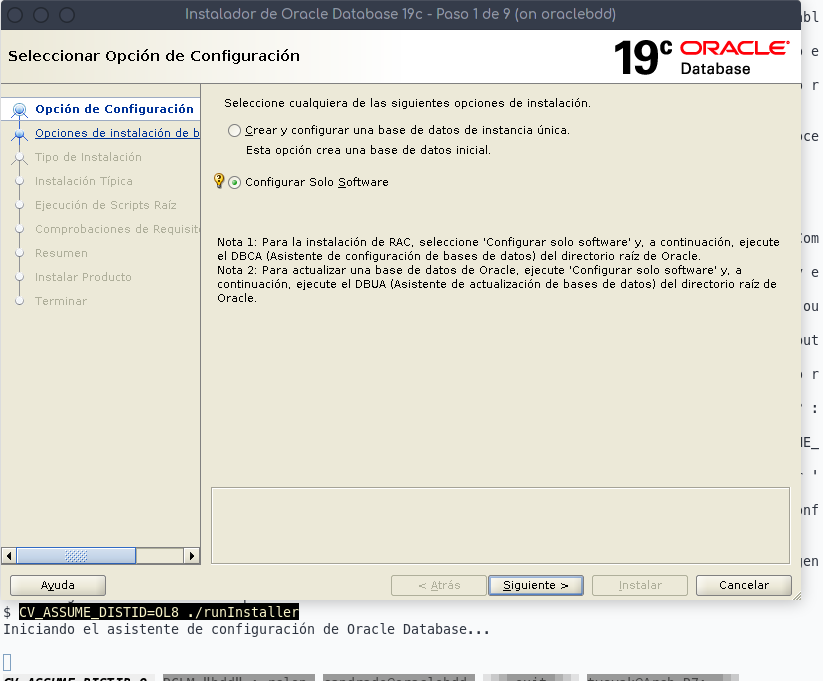
\includegraphics[width=\columnwidth]{sshx}
  \caption{Ejecución del insatalador en la máquina anfintriona usando x11 y ssh}\label{fig:sshx}
\end{figure}

\begin{figure}[H]
  \centering
  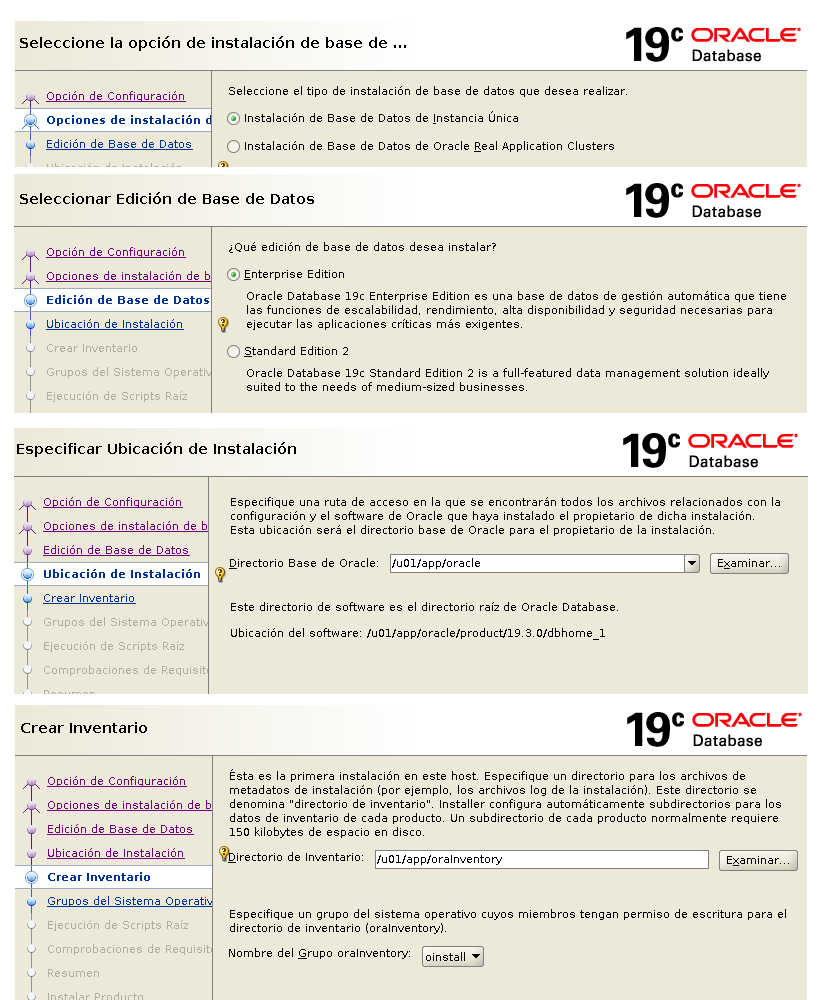
\includegraphics[width=\columnwidth]{javax1}
  \caption{Proceso de instalación de la BD 1}\label{fig:javax1}
\end{figure}

\begin{figure}[H]
  \centering
  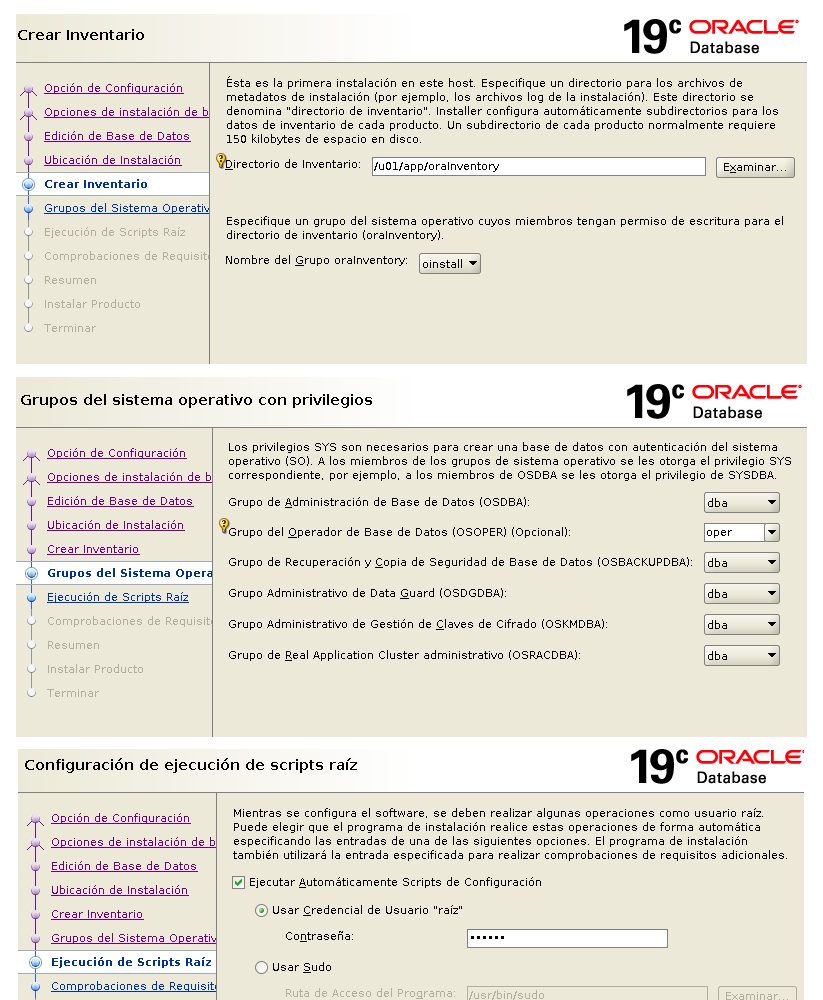
\includegraphics[width=\columnwidth]{javax2}
  \caption{Proceso de instalación de la BD 2}\label{fig:javax2}
\end{figure}

\begin{figure}[H]
  \centering
  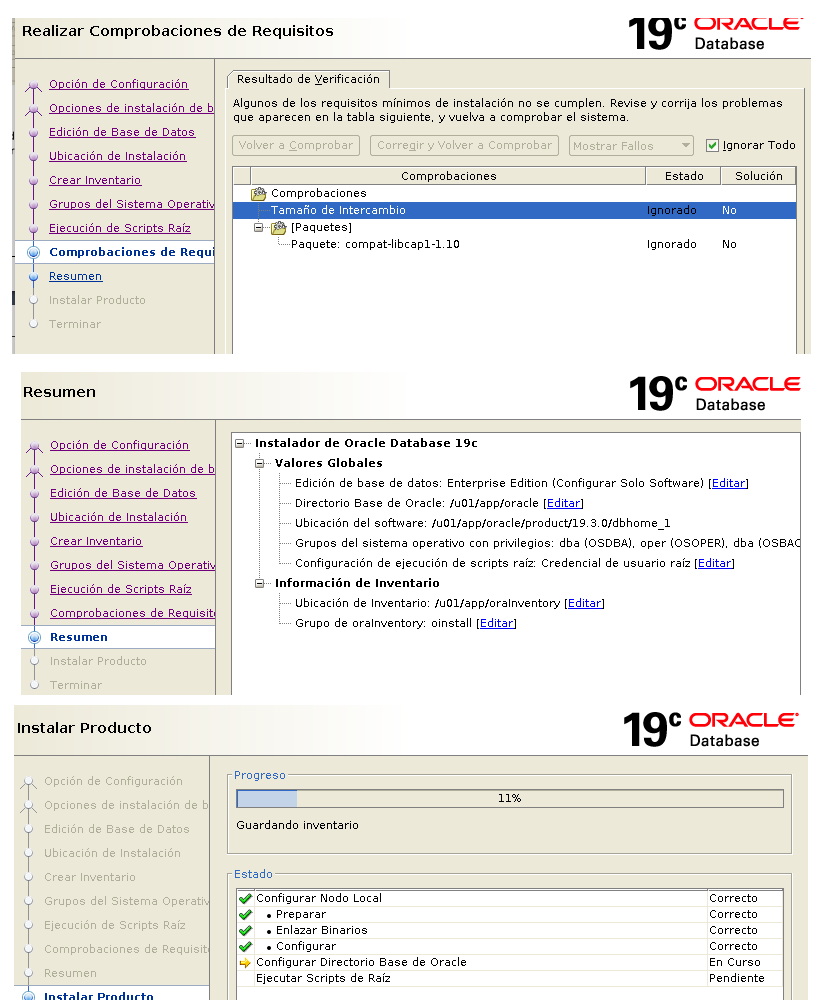
\includegraphics[width=\columnwidth]{javax3}
  \caption{Proceso de instalación de la BD 4}\label{fig:javax3}
\end{figure}

\begin{figure}[H]
  \centering
  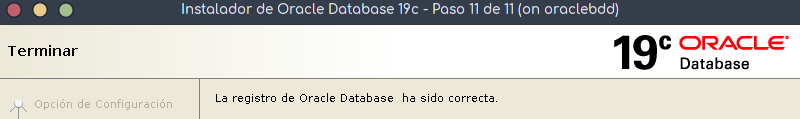
\includegraphics[width=\columnwidth]{javax4}
  \caption{Proceso de instalación de la BD 4}\label{fig:javax4}
\end{figure}

\setcounter{subsubsection}{2}
\subsubsection{Salida del script de validación}\label{sec:salida-del-script2}
A continuación se ejecuta el script de validación para finalizar la práctica:
\begin{figure}[H]
  \centering
  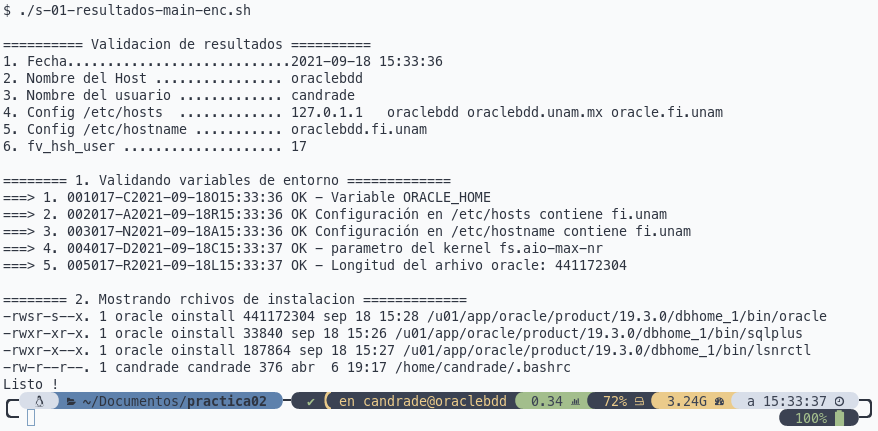
\includegraphics[width=\columnwidth]{script}
  \caption{Salida del script de validación \texttt{s-01-resultados-main-enc.sh}}\label{fig:script}
\end{figure}




\end{document}
